\documentclass[tikz,border=10pt]{standalone}

\usetikzlibrary{angles}
\begin{document}

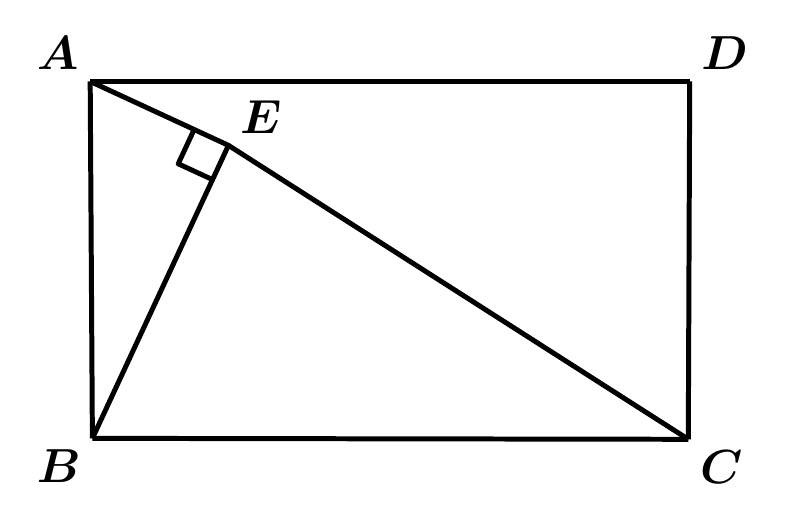
\begin{tikzpicture}[line width=1.8pt, line join=round]
\coordinate (A) at (-3.836,2.290);
\coordinate (B) at (-3.808,-2.243);
\coordinate (C) at (3.760,-2.255);
\coordinate (D) at (3.778,2.290);

\coordinate (E) at (-2.080,1.478);


\draw (A) -- (D);
\draw (D) -- (C);
\draw (B) -- (C);
\draw (B) -- (A);


\draw (A) -- (E) -- (C);


\draw (B) -- (E);


\draw pic[draw, angle radius=0.480cm] {right angle=A--E--B};


\node[above left] at (A) {\fontsize{19}{22.8}\selectfont{\boldmath$A$}};
\node[above right] at (D) {\fontsize{19}{22.8}\selectfont{\boldmath$D$}};
\node[below left] at (B) {\fontsize{19}{22.8}\selectfont{\boldmath$B$}};
\node[below right] at (C) {\fontsize{19}{22.8}\selectfont{\boldmath$C$}};
\node[above right] at (E) {\fontsize{19}{22.8}\selectfont{\boldmath$E$}};
\end{tikzpicture}
\end{document}
